\normalfont\documentclass[letterpaper,11pt]{article}
\usepackage{amsmath, amsfonts,amssymb,latexsym}
\usepackage{fullpage}
\usepackage{parskip}
\usepackage{flexisym}
\usepackage{algorithm}
\usepackage{indentfirst}
\usepackage{graphicx}
\usepackage{algorithmicx}
\usepackage{algpseudocode}
\begin{document}
\setlength{\parindent}{2ex}
\newcommand{\header}{
	\noindent \fbox{
	\begin{minipage}{6.4in}
  	\medskip
  	\textbf{CS 260 - Fundamentals of the Design and Analysis of Algorithms} \hfill \textbf{Fall 2016} \\[1mm]
  	\begin{center}
    	{\Large HomeWork 1b} \\[3mm]
  	\end{center}
	\today \hfill \itshape{Liangjian Chen}
	\medskip
	\end{minipage}}
}

\bigskip
\header

\begin{enumerate}
\item (Problem 6)\par
	A ship preference list is a list of port order by ship's chronological visit. A port preference list is a list of ship order by reverse chronological visiting time of ships. If we consider ship as man and port as women, then it becomes a stable marriage problem. Simply apply G-S algorithm in this problem, solution always exist. 
\item (Problem 7)\par
	Let's define that a conflict occur if two data streams pass through the same junction box. A output wire preference list is a list of input wire's id by the ordered of intersection point(from output wire's \textbf{downstream} to its \textbf{upstream}). A input wire preference list is a list of output wire's id by the ordered of intersection point (from input wire's \textbf{upstream} to its \textbf{downstream}).\par
	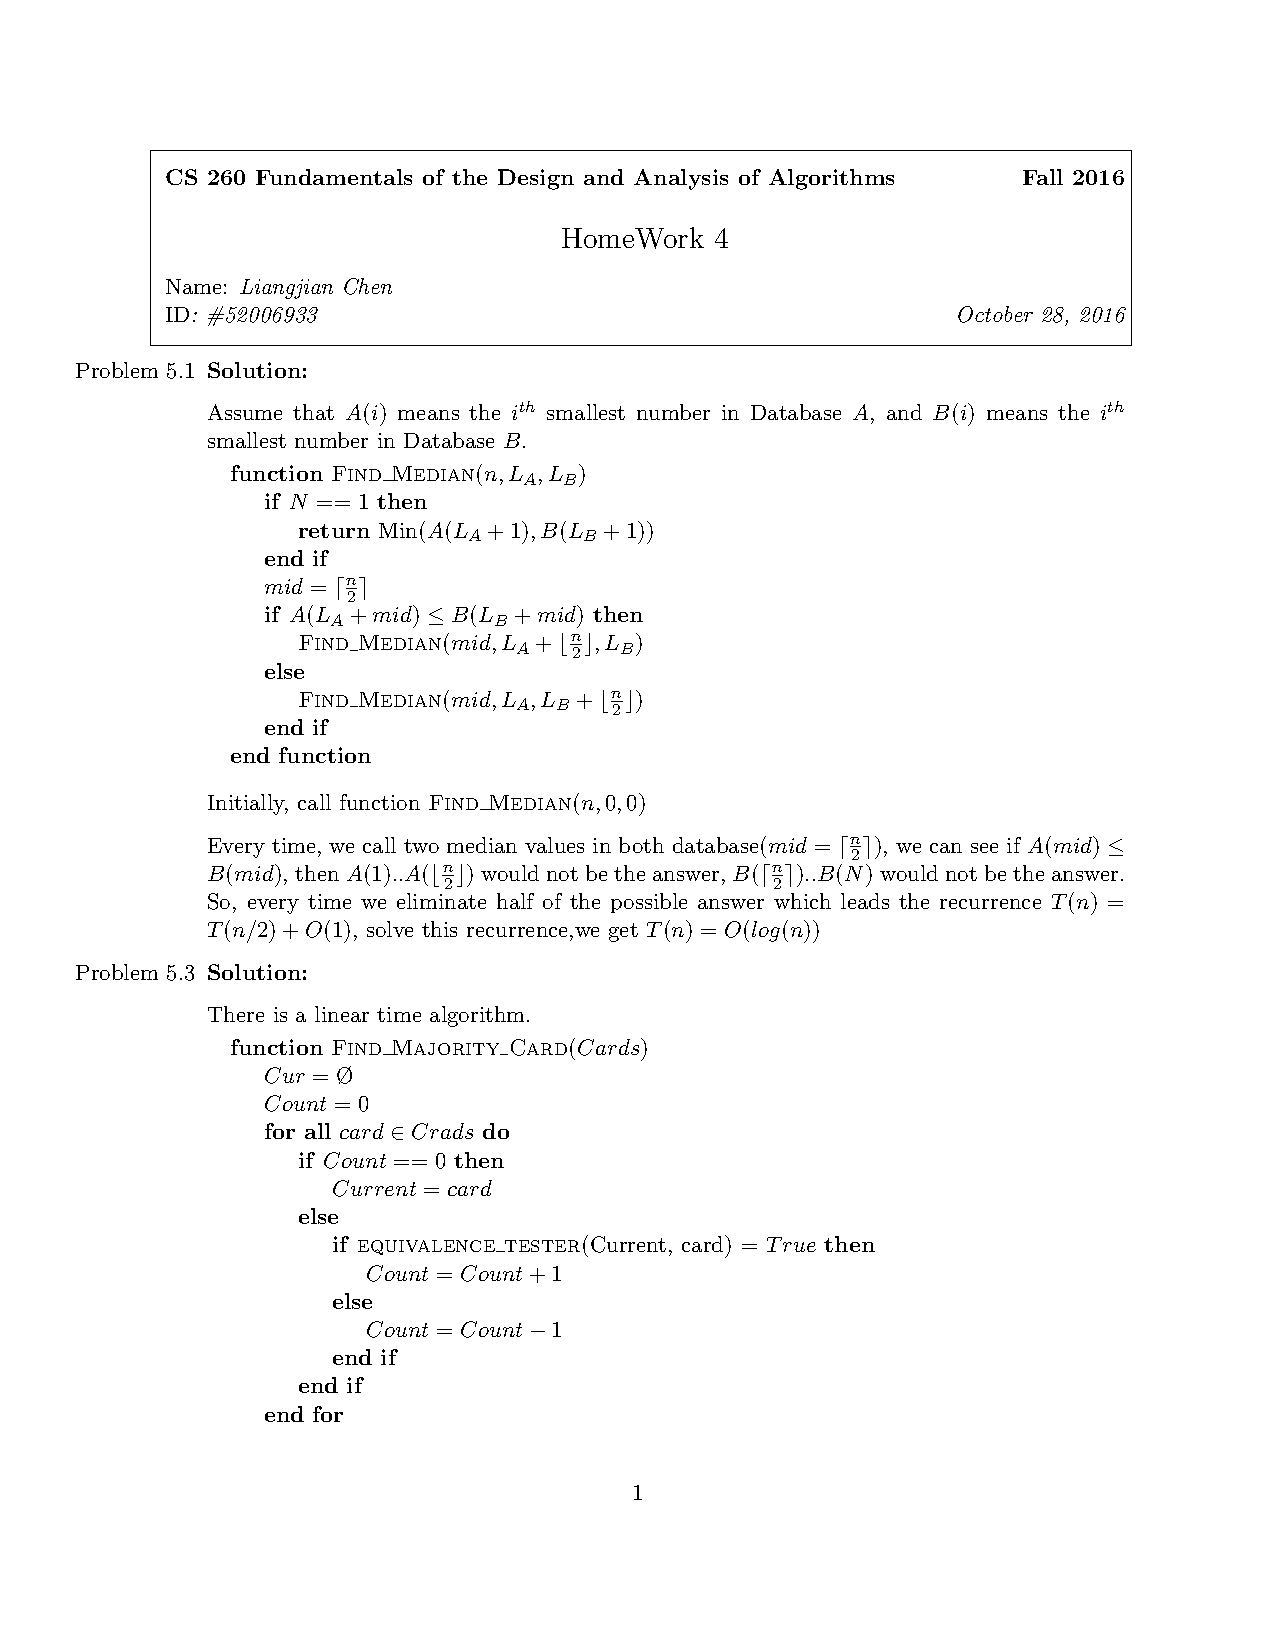
\includegraphics[width = 3in]{1.png}\par
	According to the picture, when a conflict occur, between two pairs ($I_1$,$O_1$), ($I_2$,$O_2$), $O_1$ rank higher than $O_2$ in $I_2$'s preference list. $I_2$ rank higher $I_1$ in $O_1$'s preference list. It indicate that this problem is same as stable marriage problem. So the perfect match always exist.
\item (Problem 8)\par
	The answer is yes, a woman may give a fake preference list to get a better partner. For example, there are 3 women($w_1,w_2,w_3$) and 3 men($m_1,m_2,m_3$) and their true preference list is \par

	\begin{tabular}{l | r}
	name  & preference list\\
	$w_1$ & $m_2,m_1,m_3$\\
	$w_2$ & $m_1,m_2,m_3$\\
	$w_3$ & $m_1,m_2,m_3$\\
	$m_1$ & $w_1,w_3,w_2$\\
	$m_2$ & $w_3,w_1,w_2$\\
	$m_3$ & $w_1,w_3,w_2$\\
	\end{tabular}\par
	After G-S algorithm terminating, the result is matching ($w_1,m_1$),($w_2,m_3$),($w_3,m_2$).\par
	However, if $w_1$ gives a fake preference list which is ($m_2,m_3,m_1$). Then the result is ($w_1,m_2$),($w_2,m_3$),($w_3,m_1$). Thus, $w_1$ gets her best partner $m_2$ rather than $m_1$.
\end{enumerate}

\end{document}
